\begin{frame}[t, fragile]{Histogram}
  \begin{itemize}
    \item Utilizado para explorar dados
    \item Fornece uma idea da distribuição dos dados
  \end{itemize}
  \begin{figure}
    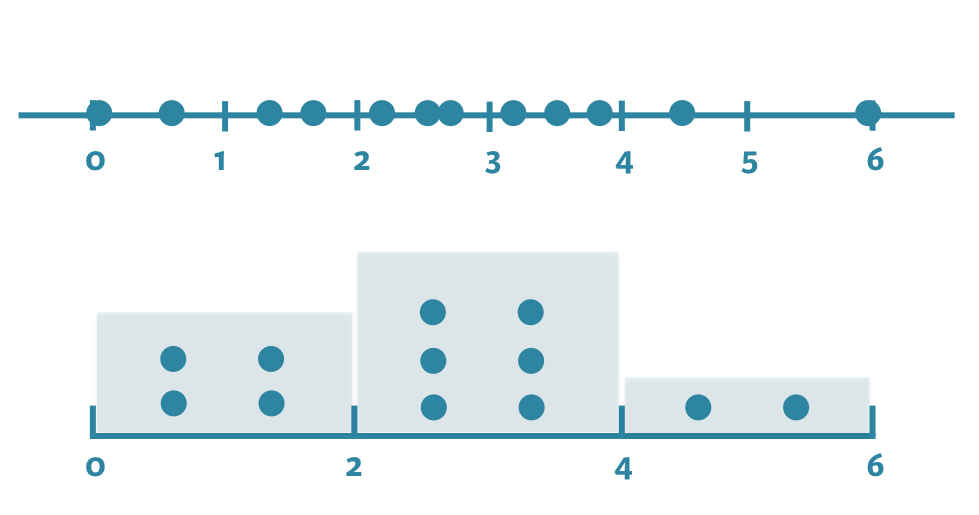
\includegraphics[scale=.40]{aula-2/figuras/matplotlib-histogram-a.png}
  \end{figure}

\end{frame}
%
\begin{frame}[t, fragile]{Histogram}
  \begin{columns}
    \begin{column}{0.5\textwidth}
        \lstinputlisting[language=python]{aula-2/codigos/matplotlib/matplotlib-histogram-1.py}  
    \end{column}

    \begin{column}{0.5\textwidth}
      \begin{center}
        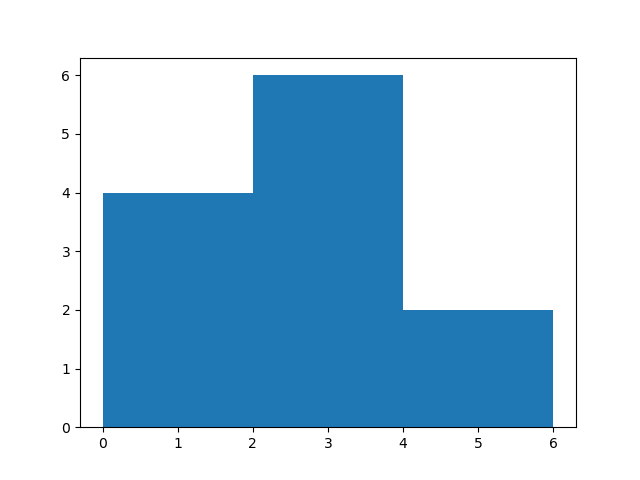
\includegraphics[scale=.40]{aula-2/figuras/matplotlib-histogram-1.png}
      \end{center}
    \end{column}
  \end{columns}
\end{frame}
%

 